\section{Expériences}
\label{sec:exp}

\subsection{Environnement}
\label{sub:env}

Afin de pouvoir éviter les obstacles le robot a besoin de connaître précisément où ils se situent autour de lui. Dans un premier temps nous devions utiliser la vision afin d'obtenir leurs coordonnées, cependant ce projet a pris un peu de retard. 
J'ai donc du utiliser un système de repérage global, comme le système de \emph{motion capture}, présent dans la salle d'expérience de robotique du LAAS.

L'utilisation est assez simple : à l'aide de 10 caméras infrarouges, le logiciel Cortex2.0 retrouve la position 3D des \emph{markers} (voir fig.\ref{fig:marker}) apposés sur les différents objets. 
Lors de la création du modèle de l'objet (voir fig.\ref{fig:objet}), les longueurs entre les \emph{markers} sont sauvegardées.


\begin{figure}[h]
\begin{center}
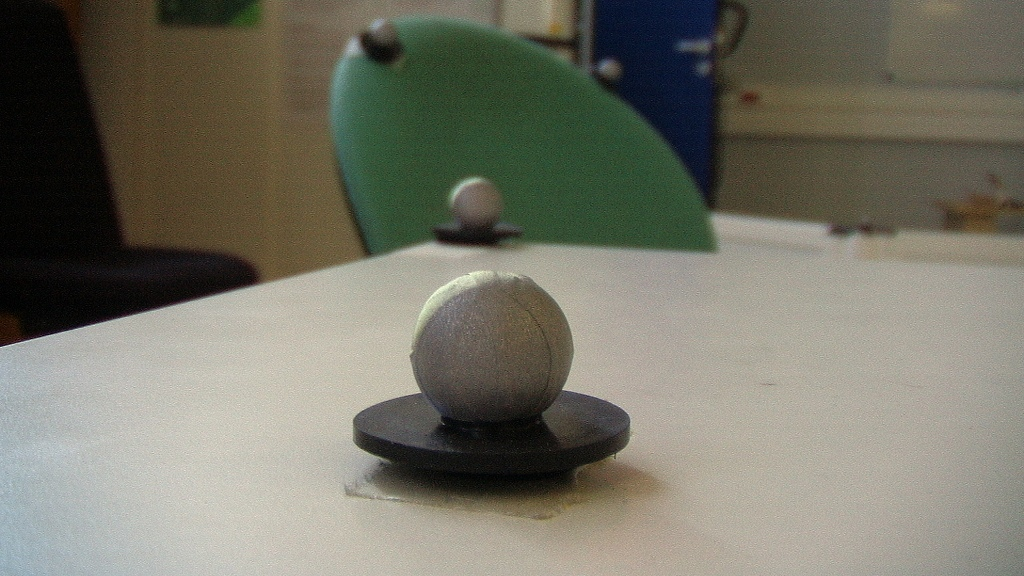
\includegraphics[width=8.0cm]{images/marker_small.jpg}
\caption{Un \emph{marker} réfléchissant les infrarouges pour la localisation.}
\label{fig:marker}
\end{center}
\end{figure}

\begin{figure}[h]
\begin{center}
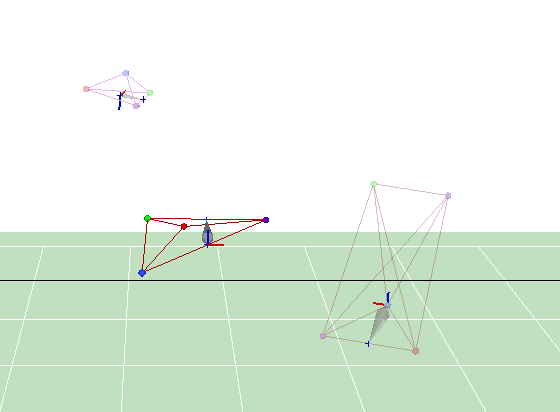
\includegraphics[width=7cm]{images/mocap.png}
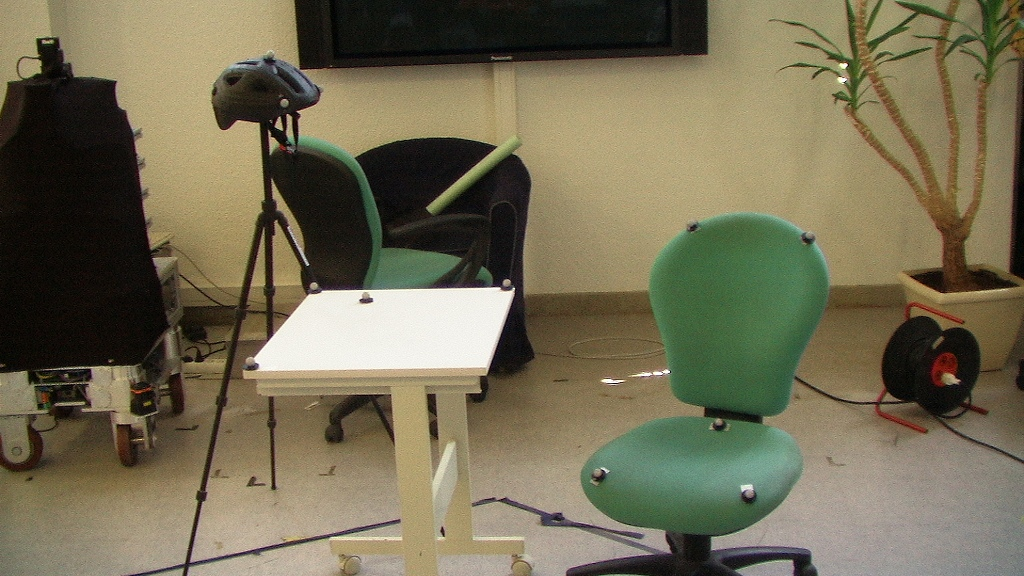
\includegraphics[width=8.5cm]{images/mocap_real_small.jpg}
\caption{Utilisation de modèles dans Cortex2.0. Ici la table est localisée à l'aide de 4 \emph{markers} disposés de manière unique dans la scène.}
\label{fig:objet}
\end{center}
\end{figure}

Les positions des objets sont ensuite déduites toutes les $5ms$ en comparant les distances entre les \emph{markers} présents dans la scènes et les distances enregistrées dans les modèles. Une fois la position de l'objet calculée, les coordonnées sont \emph{streamées} sur le réseau afin de pouvoir être lues sur tous les ordinateurs du LAAS. On peut donc avoir en temps réel les informations (position, orientation) de chacun des objets présents dans la scène.

La précision de la \emph{motion capture} est de l'ordre du centimètre et la localisation d'un objet étant effectuée à l'aide de plusieurs points, la précision sur l'emplacement d'un objet est inférieur à un centimètre.

Notre scène contient les objets suivants \emph{trackés} par la \emph{motion capture} : 
\begin{itemize}
\item Une table roulante
\item Une chaise de bureau roulante
\item Une barre à $6cm$ de haut
\item Deux tores de $1m$ de diamètre
\item Un robot HRP-2
\item Une salle (pour éviter les murs et les obstacles fixes)
\end{itemize}
\vspace{3mm}

L'espace de travail est un rectangle de $6m\times4m$ dans lequel le robot peut évoluer sans risque de collision. Cet espace est couvert par les caméras de la \emph{motion capture}, il est donc possible de déterminer les positions de tous les éléments cités précédemment. 

D'autre part, le robot doit pouvoir être maintenu en cas de chute. Pour cela, un pont roulant 3 axes est mis en place au dessus de l'espace de travail. En attendant qu'il soit auto-piloté sur la position du robot, un manipulateur doit veiller à ce que les cordes de maintien soient toujours au dessus du robot. Sans cette protection, le robot ne serait plus maintenu en cas d'accident, et les dégats pourraient être considérables lors de l'utilisation de l'arrêt d'urgence.

\subsection{Cahier des charges}
\label{sub:cdc}

Les expériences à réaliser sont réparties en quatre objectifs :
\begin{itemize}
\item Planification avec évitement et franchissement d'obstacles :\\
\emph{Le robot être être capable de trouver un chemin d'un point A à un point B en évitant ou franchissant tous les obstacles.}
\item Replanification avec les obstacles mobiles :\\
\emph{Les obstacles pourront bouger dans l'espace de travail, ils ne devront pas être placés dans les 3 prochains pas du robot, ni au dessus de la position d'arrivée du robot.}
\item Suivi de personne :\\
\emph{Le robot doit atteindre une personne portant un casque suivi par la \emph{motion capture}, il doit s'arrêter dans un carré de $1m$ autour de la position de la personne.}
\item Suivi de personne en évitant les obstacles mobiles :\\
\emph{Le robot doit être capable d'effectuer l'évitement et le suivi en même temps.}
\end{itemize}



\subsection{Résultats}
\label{sub:resultats}

L'utilisation de PQP et l'optimisation du code-source du \emph{planner} ont permis d'augmenter d'environ 30 fois la vitesse de planification. Pour un même environnement complexe, contenant des obstacles 2D et trois cubes en 3D, le temps de planification moyen est passé de $29.8s$ à $0.98s$. Ceci a permis de confirmer que l'on pouvait utiliser notre algorithme pour de la replanification en temps réel.


\begin{figure}[h]
\begin{center}
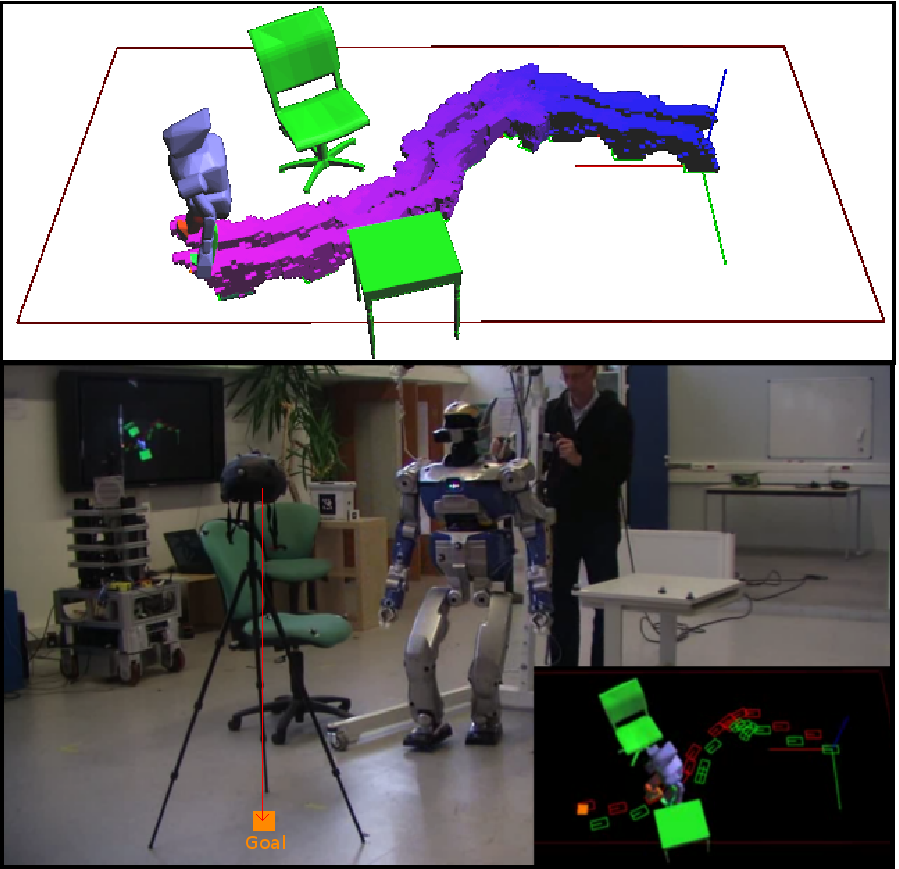
\includegraphics[width=11.0cm]{images/SweptDemo.png}
\caption{Evitement de collisions avec des obstacles complexes (>10.000 triangles). Ici, seuls les volumes balayés des jambes ont été utilisés.}
\label{fig:demo}
\end{center}
\end{figure}

Les capacités des robots humanoïdes ont bien été exploitées comme le montre la figure~\ref{fig:over} où le robot enjambe une barre. Le robot doit pouvoir naviguer dans un environnement humain, l'objectif étant de prendre des cas comme une chambre d'enfant où de nombreux objets sont disposés aléatoirement sur le sol.

\begin{figure}[h]
\begin{center}
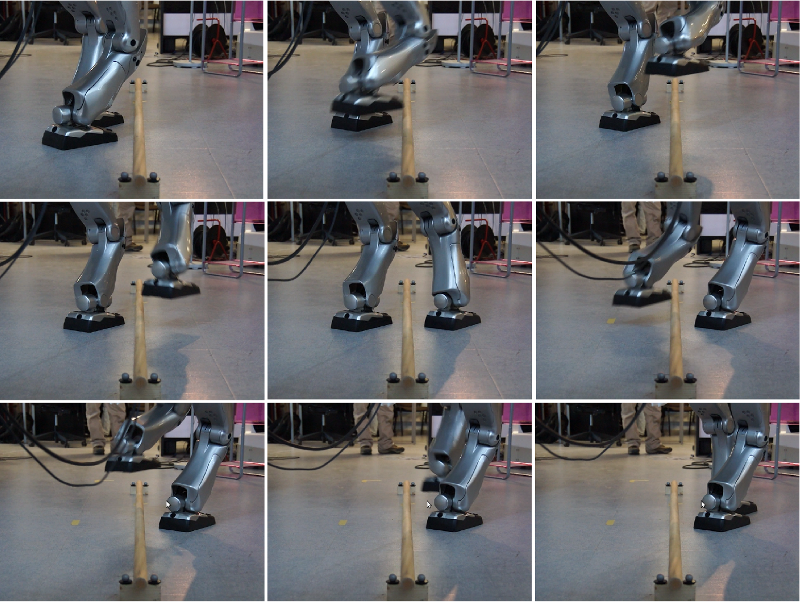
\includegraphics[width=13.0cm]{images/over_small.png}
\caption{Enjambement d'un obstacle de $8cm$ de haut lors de l'exécution d'une trajectoire planifiée par HRP-2.}
\label{fig:over}
\end{center}
\end{figure}

\newpage
